\documentclass[pdf,bluish,slideColor,colorBG]{prosper}
\hypersetup{pdfpagemode=FullScreen}
\usepackage{color}
\usepackage{graphicx}
\usepackage{amsfonts}
\usepackage{amsmath}
\def\baselinestretch{0.7}
\parindent 0.3in
\hyphenpenalty=10000
\tolerance=10000
\pagestyle{empty}

\title{Statistical nonmolecular phylogenetics: can molecular phylogenies
illuminate morphological evolution?}

\author{Joe Felsenstein}

\institution{Workshop on Molecular Evolution, MBL, Woods Hole}

\subtitle{\small \\ 25 July 2015}


\definecolor{orange}{rgb}{1.0,0.8,0.0}
\definecolor{Dandelion}{rgb}{0.8,0.4,0.3}
\definecolor{golden}{rgb}{1.0,0.75,0.2}
%\definecolor{golden}{rgb}{1.0,0.8,0.3}
\definecolor{purple}{rgb}{0.6,0.2,0.6}
\definecolor{darkblue}{rgb}{0.1,0.1,0.6}
\definecolor{yellow}{rgb}{1.0,1.0,0.0}
\definecolor{brightred}{rgb}{1.0,0.,0.0}
\definecolor{black}{rgb}{0.0,0.0,0.0}
\definecolor{white}{rgb}{1.0,1.0,1.0}
\definecolor{purple}{rgb}{0.8,0.0,0.8}

% sets backgroundcolor for whole document 
%\pagecolor{darkblue}
%\pagecolor{white}
% sets text color
%\color{yellow}
%\color{black}
% to change just a few words
% using \textcolor{color}{text}

\DeclareSymbolFont{AMSb}{U}{msb}{m}{n}
\DeclareMathSymbol{\expect}{\mathalpha}{AMSb}{'105}

\def\Prob{{\rm Prob\;}}
\def\prob{{\rm \;Prob\;}}
\def\Var{{\rm Var}}        % Var
\def\Cov{{\rm Cov}}        % Cov

\begin{document}

\maketitle

% Introduction: nonmolecular?  Why I got into it

{\parindent=0in

\begin{slide}[Replace]{Where this lecture fits in}
\bigskip

Lately, more integration of
\begin{itemize}
\item work on molecular evolution
\item work on between-species differences of measurable characters
\item work on within-species differences of measurable characters
\end{itemize}

\noindent
How can they fit together?

\end{slide}

\begin{slide}[Replace]{A standard quantitative genetics model}

\centerline{\includegraphics[width=4.0in]{quantmodel6.ydraw}}

\end{slide}

\overlays{3}{
\begin{slide}[Replace]{A model of quantitative characters on a phylogeny}

\centerline{\includegraphics[width=2in]{fig23-2.ydraw}}

\begin{itemstep}
\item Brownian motion with multiple characters with different variances and with covariation as well.
\item This started with approximating gene frequencies in the 1960s by
Anthony Edwards and Luca Cavalli-Sforza.
\item I expanded it to model quantitative characters determined by these
geness (1973, 1981, 1988).
\item Assumption that character variances and covariances
are replenished by mutation and do not change much through time.
\item The main person introducing these models was Russ Lande.
\end{itemstep}

\end{slide}
}

\begin{slide}[Replace]{Models for long-term evolution}

\bigskip

The use of quantative genetics approximations to model long-term evolution
in lineages was largely introduced by Russ Lande in the 1980s.
\bigskip

\centerline{\includegraphics[width=2in]{Lande2011.ps}}
\bigskip

Russell Lande, from his website at Imperial College, U.K., where he has been in recent years.

\bigskip

\end{slide}

\overlays{2}{
\begin{slide}[Replace] {Where do the covariances come from? }
\bigskip

\begin{itemstep}
\item {\bf Genetic covariances} (the same loci affect two or more traits).
Genetic drift or natural selection can change the gene frequencies at
these loci, and thus make correlated changes in the two traits.
\item {\bf Selective covariances} (Olof Tedin, 1926; G. Ledyard Stebbins 1950) The 
same environmental conditions can select changes in two or more traits -- even
though they may have no genetic covariance.  This source of evolutionary
covariance is widely ignored.
\end{itemstep}

\end{slide}
}


\begin{slide}[Replace] {\large Part 1:  Morphometrics and phylogenies}
\bigskip

\centerline{Fred Bookstein is a co-author on this part of the talk}
\bigskip

\begin{center}
\begin{tabular}{c c c c c}
\multicolumn{2}{c}{\includegraphics[height=0.7in]{Bookstein2009gray.ps}} & &
\multicolumn{2}{c}{\includegraphics[height=0.7in]{Joe2010.ps}} \\
\multicolumn{2}{c}{Fred Bookstein} &                                   &
\multicolumn{2}{c}{me} \\
& \multicolumn{3}{c}{\includegraphics[width=1.0in]{bookfelstree.idraw}} & \\
 &\multicolumn{3}{c}{\includegraphics[height=0.7in]{Bookenstein2010a.ps}} & \\
        &\multicolumn{3}{c}{``J. F. L. Bookenstein''} & \\
\end{tabular}
\end{center}

\centerline{(Our reconstructed common ancestor)}

\end{slide}


\begin{slide}[Replace]{How to use morphometric coordinates on phylogenies? }
\bigskip

Is it possible to simply use the coordinates of landmarks
$(x_1, y_1), (x_2, y_2), \dots, (x_p, y_p)$ as continuous
phenotypes $x_1, y_1, \dots, x_p, y_p$  using Brownian motion along a phylogeny?
\bigskip

Yes, but ...
\bigskip

We must do proper morphometrics (correct for translation? rotation?)
\bigskip

\end{slide}

\begin{slide}[Replace]{Can we superpose specimens? }

Consider two cases:

\centerline{\includegraphics[width=3.5in]{superposition.idraw}}
\bigskip

Are these different?
\end{slide}

\begin{slide}[Replace]{Why superposition is in principle impossible}

Consider two cases:

\centerline{\includegraphics[width=3.5in]{superposition.idraw}}
\bigskip

Are these different? ~~ {\Large No!}


\end{slide}

\begin{slide}[Replace]{Dealing with translation}

In effect one is centering each specimen so that
the mean of its points is at $(0, 0)$.  (The
assumption is that the horizontal and vertical
placement of the specimen on the digitizer is
not useful information).
\bigskip

This has the effect of dropping two degrees of
freedom so that each specimen now has $2p-2$
coordinates.  It now ``lives'' in a $(2p-2)$-dimensional
space.
\bigskip

\end{slide}

\begin{slide}[Replace]{The annoying issue of rotation}
\bigskip

\centerline{\includegraphics[width=2.5in]{rotation.idraw}}
\bigskip

Sadly, there is no corresponding transform that
tosses out rotation, as there is for translation.
\bigskip

\end{slide}

\begin{slide}[Replace]{Degrees of freedom and other transforms}
\bigskip

In the morphometrics literature this is dealt with by a Procrustes Transform.
\bigskip

Fred and I estimate rotations separately for each specimen:
choose the angles of rotation of all but the first specimen ($\theta_2, \theta_3,
\dots, \theta_p$) to maximize the resulting likelihood.
\bigskip

All of these reduce the degrees of freedom of each specimen by 3, to $2p-3$.
\medskip

But does this mean that the multivariate density function does not
exist?  No, it does exist, just in a $(2p-3)$-dimensional subspace.
\medskip

\begin{center}
\fbox{
\parbox[c]{4in}{
In that space, all the usual machinery of the phylogenetic
comparative method is available: contrasts to evaluate
covariation of characters, reconstruction of ancestors, etc.
}}
\end{center}

\end{slide}

\begin{slide}[Replace]{A simulation test}
{\ptsize{8}
\begin{enumerate}
\itemsep -3pt
\item Generate 50 100-species trees by a pure birth process
\item For each evolve 100 forms by (covarying) Brownian Motion up the
tree
\item These are the true covariances:
\end{enumerate}

\centerline{\includegraphics[width=2.2in]{urfish2.idraw}}

\begin{itemize}
\itemsep -3pt
\item All 10 landmarks move by independent and equal Brownian Motion of the
coordinates with variance (per unit branch length) of 0.001, {\it plus}
\item the vertical coordinate of the pectoral fin and the two coordinates
of the top of the tail move in a perfectly correlated change with variance
0.003.
\end{itemize}

}
\end{slide}

\begin{slide}[Replace]{20 of the 100 fishes from data set \#2, centered and rotated}
\bigskip

\centerline{\includegraphics[width=3in]{fishes28.2.idraw}}

\end{slide}

\begin{slide}[Replace]{20 of the 100 fishes from data set \#2, also rescaled}
\bigskip

\centerline{\includegraphics[width=3in]{fishes28.2shape.idraw}}

\end{slide}

\begin{slide}[Replace]{First PC 1 for data set \#2}
\bigskip

\centerline{\includegraphics[width=3in]{fishes28.2.formandpc.idraw}}
\bigskip

This principal component shows both size changes and the fin extensions,
and it is not easy to see which is which.

\end{slide}

\begin{slide}[Replace]{First shape PC 1 for data set \#2}
\bigskip

\centerline{\includegraphics[width=3in]{fishes28.2shape.formandpc.idraw}}
\bigskip

Now we've inferred a scale (size) component and removed it from the
covariances, and then taken the first PC of the residual on size.  We
can see the fin component more clearly.

\end{slide}

\begin{slide}[Replace]{Making the first shape PC sparser by ``medianizing'' }
\bigskip

\centerline{\includegraphics[width=3in]{fishes28.2shape.formandpcmed.idraw}}
\bigskip

To make PC1 be sparses we can add in a little location (not forcing the
changes to maintain the centroid supeposition).  This is done by subtracting
from the $\mathsf{~x~}$ components, their median, and similarly for the
$\mathsf{~y~}$ components.  So it minimizes the $\mathsf{L^1}$ norm of the
PC coefficients.

The result is very clear.

\end{slide}

\begin{slide}[Replace]{What do we get from the Morphometric Consensus? }

Using a Procrustes superposition and assuming the forms are i.i.d. and then
computing principal components:
\medskip

\centerline{\includegraphics[width=3in]{fishes28.2proc.formandpc.idraw}}

... we get a not-as-clear result with some size still there -- we have ignored the tree and taken out size by standardizing centroid size, which is affected more by the fin component in the MMC methods.

\end{slide}

\begin{slide}[Replace] {Part 2: Fossils and phylogenies}
\bigskip

(see also Tracy Heath's talk later today -- her method and this one are
quite compatible)
\bigskip

There is also a very similar approach published recently by Revell et al. (2015)

\end{slide}

\begin{slide}[Replace]{Present methods for calibration}

\centerline{\includegraphics[width=1.8in]{calibrate2.idraw}} 
\medskip

Can take a fossil to indicate a bound on how recently
a common ancestor was present.  Use various priors on
how much earlier or how much more recently.
\bigskip

But there is another way, which is being explored by
me and (independently) by Alexander Pyron (2011) and by Fredrik Ronquist et
al. (2012)

\end{slide}

\begin{slide}[Replace]{Another way of using fossils}

\centerline{\includegraphics[width=3.5in]{fossils1a.ydraw}}
\bigskip

\centerline{Infer tree of present-day species from molecular sequences}

\end{slide}

\begin{slide}[Replace]{Using fossils}

\centerline{\includegraphics[width=3.5in]{fossils1b.ydraw}}
\bigskip

\centerline{Infer covariances of morphology using it, present-day species}

\end{slide}

\begin{slide}[Replace]{Using fossils}

\centerline{\includegraphics[width=3.5in]{fossils1c.ydraw}}
\bigskip

\centerline{Infer placement of fossil species using their data}

\end{slide}

\begin{slide}[Replace]{Using fossils}

\centerline{\includegraphics[width=3.5in]{fossils2a.ydraw}}
\bigskip

\centerline{Use fossil and present-day morphology, covariances, tree,}
\centerline{ also stratigraphic models}

\end{slide}

\begin{slide}[Replace]{Using fossils}

\centerline{\includegraphics[width=3.5in]{fossils2b.ydraw}}
\bigskip

\centerline{Use fossil and present-day morphology, covariances, tree,}
\centerline{ also stratigraphic models}

\end{slide}

\begin{slide}[Replace]{Using fossils}

\centerline{\includegraphics[width=3.5in]{fossils2c.ydraw}}
\bigskip

\centerline{Use fossil and present-day morphology, covariances, tree,}
\centerline{ also stratigraphic models}

\end{slide}

\begin{slide}[Replace]{Using fossils}

\centerline{\includegraphics[width=3.5in]{fossils2d.ydraw}}
\bigskip

\centerline{Use fossil and present-day morphology, covariances, tree,}
\centerline{ also stratigraphic models}

\end{slide}

\begin{slide}[Replace]{Using fossils}

\centerline{\includegraphics[width=3.5in]{fossils2e.ydraw}}
\bigskip

\centerline{Use fossil and present-day morphology, covariances, tree,}
\centerline{ also stratigraphic models}

\end{slide}

\begin{slide}[Replace]{Using fossils}

\centerline{\includegraphics[width=3.5in]{fossils2f.ydraw}}
\bigskip

\centerline{Use fossil and present-day morphology, covariances, tree,}
\centerline{ also stratigraphic models}

\end{slide}

\begin{slide}[Replace]{Using fossils}

\centerline{\includegraphics[width=3.5in]{fossils2g.ydraw}}
\bigskip

\centerline{Use fossil and present-day morphology, covariances, tree,}
\centerline{ also stratigraphic models}

\end{slide}

\begin{slide}[Replace]{Using fossils}

\centerline{\includegraphics[width=3.5in]{fossils2h.ydraw}}
\bigskip

\centerline{Use fossil and present-day morphology, covariances, tree,}
\centerline{ also stratigraphic models}

\end{slide}

\begin{slide}[Replace]{Using fossils}

\centerline{\includegraphics[width=3.5in]{fossils2i.ydraw}}
\bigskip

\centerline{Use fossil and present-day morphology, covariances, tree,}
\centerline{ also stratigraphic models}

\end{slide}

\begin{slide}[Replace]{Using fossils}

\centerline{\includegraphics[width=3.5in]{fossils2j.ydraw}}
\bigskip

\centerline{Use fossil and present-day morphology, covariances, tree,}
\centerline{ also stratigraphic models}

\end{slide}

\begin{slide}[Replace]{Using fossils}

\centerline{\includegraphics[width=3.5in]{fossils2k.ydraw}}
\bigskip

\centerline{Use fossil and present-day morphology, covariances, tree,}
\centerline{ also stratigraphic models}

\end{slide}

\begin{slide}[Replace]{Using fossils}

\centerline{\includegraphics[width=3.5in]{fossils2l.ydraw}}
\bigskip

\centerline{Use fossil and present-day morphology, covariances, tree,}
\centerline{ also stratigraphic models}

\end{slide}

\begin{slide}[Replace]{Using fossils}

\centerline{\includegraphics[width=3.5in]{fossils2m.ydraw}}
\bigskip

\centerline{Use fossil and present-day morphology, covariances, tree,}
\centerline{ also stratigraphic models}

\end{slide}

\begin{slide}[Replace]{Using fossils}

\centerline{\includegraphics[width=3.5in]{fossils2n.ydraw}}
\bigskip

\centerline{Use fossil and present-day morphology, covariances, tree,}
\centerline{ also stratigraphic models}

\end{slide}

\begin{slide}[Replace]{Using fossils}

\centerline{\includegraphics[width=3.5in]{fossils2o.ydraw}}
\bigskip

\centerline{Use fossil and present-day morphology, covariances, tree,}
\centerline{ also stratigraphic models}

\end{slide}

\begin{slide}[Replace]{A simple result}
\bigskip

The upshot is that to find the maximum likelihood placement of a fossil
lineage, we
\begin{itemize}
\item Hook it up somewhere
\item Obtain the contrasts for that tree
\item Infer the phylogenetic covariances of the characters from the contrasts
\item The log-likelihood for this placement is (a constant plus) $~\mathsf{-(n-1)/2~}$ times
the log of the determinant of the covariance matrix, minus a penalty which
depends on the sum of the logs of the standard deviations of the contrasts.
\end{itemize}

So we minimize the determinant plus penalty to find the best placement.  We can
consider whether we can do likelihood ratio tests, too, at least for
placement within a single branch.

\end{slide}

\begin{slide}[Replace]{An example: the true tree with F a fossil species}
\bigskip

\centerline{\includegraphics[width=4in]{fossil.idraw}}

\end{slide}

\begin{slide}[Replace]{Traffic-light colors shows where fossil can be placed}
\bigskip

\centerline{\includegraphics[width=4in]{fossil2.idraw}}
\bigskip

Green = within 1 log-likelihood unit, Orange = within 2 units, Red = lower than
that.  Green arrow is the ML placement.  Gray placements are ruled out by
date of the fossil.

\end{slide}

\begin{slide}[Replace]{Calibrating the molecular clock}
\bigskip

\centerline{\includegraphics[width=3in]{fossils3a.ydraw}}
\bigskip

\noindent
Molecular trees don't usually have branch lengths on a time scale,
and we need that.  How to infer the calibration of the clock?

\end{slide}

\begin{slide}[Replace]{Calibrating the molecular clock}

\centerline{\includegraphics[width=4in]{fossil3.idraw}}

For example if (not a real example) the placement of F turned out to be
as shown, with the branch length shown in red, that in turn scales the
whole molecular tree, as we know the time of F.

\end{slide}

\begin{slide}[Replace]{Calibrating the molecular clock}
\bigskip

\centerline{\includegraphics[width=3in]{fossils3b.ydraw}}
\bigskip

\noindent
There will be two quantities to infer, the scaling of the molecular tree on
the time scale, and the placement of the connection to the fossil.  We make an
ML estimate and accept other values that are not rejected by a Likelihood Ratio
Test with 2 degrees of freedom.

\end{slide}

\overlays{4}{
\begin{slide}[Replace]{A qualification}
\bigskip

\begin{itemstep}
\item The present method takes the molecular tree as known.
\item Uncertainty in it could be modelled by doing the analysis multiple
times on bootstrap samples (or Bayesian posterior samples) of the tree
estimates.
\item Pyron and Ronquist both use a more comprehensive ``total evidence''
approach of allowing the morphological data to influence Bayesian inference
of the tree.
\item I suspect this will have little effect if there is a lot of molecular
data, so I am sticking with this approach.
\end{itemstep}


\end{slide}
}

\begin{slide}[Replace] {Part 3:  A threshold model for 0/1 characters}
\bigskip

\bigskip

(This was published in {\it American Naturalist} in 2012)
\bigskip
 
\end{slide}

\begin{slide}[Replace]{Current methods for statistical treatment of 0/1 characters}

Pagel (1994) and Lewis (2001) treat such data with 

\centerline{\includegraphics[width=1.3in]{lewis.idraw}}
\noindent

Pagel allows inference of whether change is correlated, on a known tree.
Lewis infers the tree, but does not allow for correlations among characters.

Neither takes into account contributions to a 0/1 character
from multiple underlying loci.

\end{slide}

\begin{slide}[Replace]{The threshold model}

\centerline{A relevant model was invented in 1934 by}
\bigskip

\centerline{\includegraphics[width=1.5in]{wrightgp3.ps}}
\bigskip

\centerline{Sewall Wright (1889-1988)}

\centerline{shown here in 1954}

\end{slide}

\begin{slide}[Replace]{The threshold model}

\centerline{A relevant model was invented in 1934 by}
\bigskip

\centerline{\includegraphics[width=1.5in]{wrightgp3.ps}}
\bigskip

\centerline{Sewall Wright (1889-1988)}

\centerline{~}

\centerline{rumor has it he then absent-mindedly}
\centerline{erased the board with the guinea pig}

\end{slide}

\begin{slide}[Replace]{Sewall Wright, at the University of Chicago, 1928}

\begin{center}
\begin{tabular}{c c}
\includegraphics[height=2in]{wright1928.ps} &
\includegraphics[height=2in]{wrightabsent2013b.ps}\\
In 1928 &  Same place \\
& in May, 2013\\
\end{tabular}
\end{center}

\end{slide}

\begin{slide}[Replace]{The threshold model}

\centerline{\includegraphics[width=2.3in]{wrightthreshold2.ps}}
\bigskip

\centerline{Sewall Wright (1934), guinea pig digit number}

\centerline{(from Wright's follow-up 1934 second paper)}

\end{slide}

\begin{slide}[Replace]{The threshold model on a tree}

\centerline{\includegraphics[height=1.8in]{threshtree.ydraw}}

\end{slide}

\begin{slide}[Replace]{Computing the likelihood}

With two species, one character:\\

\centerline{\includegraphics[height=1.3in]{threshold2.ydraw}}

Disadvantages:
\medskip

Quite hard to compute likelihoods: need to compute area in a corner of
a correlated multivariate normal distribution.
\medskip

With 5 species, one character:
{\hspace{-0.1in}\[
\renewcommand{\arraystretch}{1.7}
\begin{array}{c l}
\mathsf{L} & \mathsf{ = \ \prob(1, 1, 0, 1, 1)}\\
 & \mathsf{ \ = \ \displaystyle{\int_0^\infty \int_0^\infty \int_{-\infty}^0 \int_0^\infty\int_0^\infty} \varphi (x_1, x_2, x_3, x_4, x_5\;|\;{\rm Tree})\;dx_1\;dx_2\;dx_3\;dx_4\;dx_5
}
\end{array}
\]
}

\end{slide}

% \begin{slide}[Replace]{Likelihoods under the threshold model on a tree}
% 
% To compute the likelihood for a tree under the threshold
% model with $p$ characters, want to compute:
% 
% \[
% \begin{array}{l l}
% \mathsf{L \ =} & \mathsf{\int_c^\infty \int_{-\infty}^c \dots \int_c^\infty 
% \;|{\bf V}|^{-1} (2\pi)^{-np / 2}}\\
% & \\
 % & \mathsf{\ \ \times \exp\left(-\frac{1}{2}\;({\bf x}-{\bf \mu})^t\;{\bf V}^{-1}\;({\bf x}-{\bf \mu})\;\right)\;dx_{11}\;dx_{12} \dots dx_{np}}
% \end{array}
% \]
% 
% where $\mathsf{\bf \mu}$ is the appropriate vector of means, and
% \[
% \mathsf{{\bf V} \ = \ {\bf A} {\bf \otimes} {\bf T}}
% \]
% involves the tree and the ``evolutionary" covariance matrix of
% the characters.
% \bigskip
% 
% In other words, the probability density of the (unknown) liabilities
% gets integrated over the region of their values that corresponds to the
% observed discrete characters.
% 
% \end{slide}
% 

\begin{slide}[Replace]{MCMC on liabilities}

\centerline{\includegraphics[height=2.8in]{threshmc1.ydraw}}

\end{slide}

\begin{slide}[Replace]{MCMC on liabilities: Gibbs sampling in the interior}

\centerline{\includegraphics[height=2.8in]{threshmc2.ydraw}}

\end{slide}

\begin{slide}[Replace]{MCMC on liabilities: result of Gibbs sampling}

\centerline{\includegraphics[height=2.8in]{threshmc3.ydraw}}

\end{slide}

\begin{slide}[Replace]{MCMC on liabilities: rejection at tips}

\centerline{\includegraphics[height=2.8in]{threshmctip.ydraw}}

\end{slide}

\begin{slide}[Replace]{An example}

\centerline{\includegraphics[height=3in]{threshex1.idraw}}

\end{slide}

\begin{slide}[Replace]{An example}

\centerline{\includegraphics[height=3in]{threshex2.idraw}}

\end{slide}

\begin{slide}[Replace]{An example}

\centerline{\includegraphics[height=3in]{threshex3.idraw}}

\end{slide}

\begin{slide}[Replace]{An example}

\centerline{\includegraphics[height=3in]{threshex4.idraw}}

\end{slide}

\begin{slide}[Replace]{An example}

\centerline{\includegraphics[height=3in]{threshex5.idraw}}

\end{slide}

\begin{slide}[Replace]{An example}

\centerline{\includegraphics[height=3in]{threshex6.idraw}}

\end{slide}

\begin{slide}[Replace]{An example}

\centerline{\includegraphics[height=3in]{threshex7.idraw}}

\end{slide}

\begin{slide}[Replace]{An example}

\centerline{\includegraphics[height=3in]{threshex8.idraw}}

\end{slide}

\begin{slide}[Replace]{An example}

\centerline{\includegraphics[height=3in]{threshex9.idraw}}

\end{slide}

\begin{slide}[Replace]{An example}

\centerline{\includegraphics[height=3in]{threshex9.idraw}}

\end{slide}

\begin{slide}[Replace]{An example}

\centerline{\includegraphics[height=3in]{threshex10.idraw}}

\end{slide}

\begin{slide}[Replace]{An example}

\centerline{\includegraphics[height=3in]{threshex11.idraw}}

\end{slide}

\begin{slide}[Replace]{An example}

\centerline{\includegraphics[height=3in]{threshex12.idraw}}

\end{slide}

\begin{slide}[Replace]{An example}

\centerline{\includegraphics[height=3in]{threshex13.idraw}}

\end{slide}

\begin{slide}[Replace]{A 3-character simulation}

\vspace{-0.13in}

\includegraphics[height=3.3in]{100tips.idraw}

\end{slide}

\begin{slide}[Replace]{A 3-character simulation}
\bigskip

\begin{center}
For these true covariances:\\
\[
\left[\begin{array}{c c c}
\mathsf{1.64} & \mathsf{0.8} & \mathsf{0} \\
\mathsf{0.8} & \mathsf{1.36}  & \mathsf{-0.6} \\
\mathsf{0} & \mathsf{-0.6} & \mathsf{1}
\end{array}\right]
\]

100 data sets with 100-species trees were analyzed.
\end{center}

\end{slide}

\begin{slide}[Replace]{Inferred correlation coefficients}
\bigskip

\begin{center}
\begin{tabular}{c c c}
  & character 1 & character 2 \\
\hline
\parbox[b]{1.0in}{character 1\\ \\} & \rule{0pt}{0.6in} & \\
\parbox[b]{1.0in}{character 2\\ \\} & \includegraphics[width=1.4in]{r12.idraw} & \\
\parbox[b]{1.0in}{character 3\\ \\} & \includegraphics[width=1.4in]{r13.idraw} &
\includegraphics[width=1.4in]{r23.idraw} \\
\end{tabular}
\end{center}

\end{slide}

\overlays{3}{
\begin{slide}[Replace]{What about QTLs? }

\begin{itemstep}
\item We can integrate this work with
QTL inference.
\item Not only identify QTLs, but to see them change across species,
including some QTLs causing variation within some species, some within
others.
\item Could even allow us to infer on which of two
correlated characters the selection really acted.
\end{itemstep}

\end{slide}
}

\begin{slide}[Replace]{The Reunion}
\bigskip

\begin{itemize}
\item For the last 40-50 years population-genetic work within species has
been (mostly) isolated from work on molecular evolution between species.
\item Now we are in a gradual Reunion of these two lines of work ({\it
not a New Synthesis, though}) as observations can be made that connect
them (coalescents across species boundaries, Ds/Dn inferences, etc.)
\item As this happens, Russ Lande's vision will become more and more of
a reality -- quantitative genetics will become directly relevant to
multi-species evolutionary biology.
\end{itemize}

More generally we are seeing increased connections between
\begin{itemize}
\item Within- and between-species work
\item Morphological and genomic studies
\item Paleontological and neontological studies
\end{itemize}
\end{slide}

\overlays{2}{
\begin{slide}[Replace]{What we can ... and cannot ... infer}

\begin{itemstep}
\item BUT ... we have limited power from any one sample of species.
Biologists must learn to accept that, and find ways to propagate that
uncertainty through the analysis that flow from these inferences.
We cannot (ever!) have a Fly-On-The-Wall account of evolution.
\item Furthermore we must always be sensitive to the limits of our
models -- as we expand the tree to less related groups, the models
are called severely into question.
\end{itemstep}

\end{slide}
}

\begin{slide}[Replace]{An advertisement}
\bigskip

\begin{center}
\fbox{
\parbox[t]{3in}{
Steve Arnold and I are running a course on Evolutionary Quantitative Genetics
this summer (as we have done the previous four years), this
time at the National Institute for Mathematical and Biological Synthesis
(NIMBioS) in Knoxville.  It starts on Monday, August 10.
\bigskip

Other faculty include Patrick Carter, Adam Jones, Michael Whitlock, 
Em\'ilia Martins, Liam Revell, and Brian O'Meara.
\bigskip

Next year it may (or may not) happen again.
}
}


\end{center}

\end{slide}


\begin{slide}[Replace]{Thanks to ... }
\bigskip

\begin{center}
\begin{tabular}{c c c }
\includegraphics[width=0.5in]{nsf.ps} &
\includegraphics[width=0.5in]{nigms.ps} &
\includegraphics[width=0.7in]{foundation.ps}\\
& & \\
NSF & NIH NIGMS & Felsenstein / Rudd \\
    &           & family funds \\
for several & for several past &          \\
grants to me & grants to me & (more and  \\
& and Mary Kuhner & more necessary) \\
& & \\
\end{tabular}
\end{center}

\end{slide}

\begin{slide}[Replace]{References}

{~~}\hspace{25pt}\parbox[t]{4in}{\parindent=-15pt

Lande, R.  1976.  Natural selection and random genetic drift in phenotypic
evolution.  {\it Evolution} {\bf 30 (2):} 314-334. \textcolor{purple}{\bf [One
of Russ's major papers using the constant-variances approximation]}

Stebbins, G. L.  1950. Variation and Evolution in Plants.  Columbia University
Press, New York. \textcolor{purple}{\bf [Describes selective covariance and
cites Tedin (1926) for it]}

Pyron, R. A.  2011.  Divergence time estimation using fossils as terminal taxa
and the origins of Lissamphibia. {\it Systematic Biology} {\bf 60:} 466-481.
\textcolor{purple}{\bf [Pioneering paper on using morphology and molecules to place fossils and date divergences]}

Ronquist, F., S. Klopfstein, L. Vilhelmsen, S. Schulmeister, D. L. Murray, and
A. P. Rasnitsyn.  2012.  A total-evidence approach to dating with fossils,
applied to the early radiation of the Hymenoptera.  {\it Systematic Biology},
Early Access, 10.1093/sysbio/sys058
\textcolor{purple}{\bf [Another pioneering paper on using morphology and molecules to place fossils and date divergences]}


}

\end{slide}

\begin{slide}[Replace]{References}

{~~}\hspace{25pt}\parbox[t]{4in}{\parindent=-15pt

Revell, L. J., D. L. Mahler, R. G. Reynolds, and G. J. Slater. 2015. Placing
cryptic, recently extinct, or hypothesized taxa into an ultrametric phylogeny
using continuous character data: A case study with the lizard {\it Anolis
roosevelti}. {\it Evolution} {\bf 69:} 1027-1035. \textcolor{purple}{\bf
[Equivalent to the approach advocated here -- computations different in detail
but results should be the same]}

Lewis, P. O.  2001.  A likelihood approach to estimating phylogeny from
discrete morphological character data.  {\it Systematic Biology} 50: 913-925.
\textcolor{purple}{\bf [Uses 0/1 stochastic process to infer morphological
phylogenies]}

Pagel, M.  1994. Detecting correlated evolution on phylogenies: A general
method for the comparative analysis of discrete characters.
{\it Proceedings of the Royal Society of London Series B Biological
Sciences.}  {\bf 255:} 37-45. \textcolor{purple}{\bf [0/1 stochastic model for discrete
characters]}

Wright, S. 1934. An analysis of variability in number of digits in an 
inbred strain of guinea pigs.  {\it Genetics} {\bf 19:} 506-536.
\textcolor{purple}{\bf [The threshold model for discrete traits]}

Falconer, D. S.  1965.  The inheritance of liability to certain diseases,
estimated from the incidence among relatives.  {\it Annals of Human Genetics}
{\bf 29:} 51-76. \textcolor{purple}{\bf [Threshold model applied to human diseases]}

}

\end{slide}

\begin{slide}[Replace]{References}

{~~}\hspace{25pt}\parbox[t]{4in}{\parindent=-15pt
Felsenstein, J.  1988.  Phylogenies and quantitative characters.  
{\it Annual Review of Ecology and Systematics} {\bf 19:} 445-471. \textcolor{purple}{\bf [Review
with mention of usefulness of threshold model]}

Felsenstein, J.  2002.  Quantitative characters, phylogenies, and morphometrics.pp. 27-44 in ``Morphology, Shape, and Phylogenetics", ed. N. MacLeod.
Systematics Association Special Volume Series 64.  Taylor and Francis, London.
\textcolor{purple}{\bf [Review repeating 1988 material and going into some more detail on the
question of threshold models.]}

Felsenstein, J.  2004.  {\it Inferring Phylogenies.}  Sinauer Associates,
Sunderland, Massachusetts. \textcolor{purple}{\bf Mentions threshold model}
\medskip


Felsenstein, J.  2005.  Using the quantitative genetic threshold model for
inferences between and within species.  {\it Philosophical Transactions of the
Royal Society of London, series B} {\bf ~360:} 1427-1434.
\textcolor{purple}{\bf [The threshold
project in a slightly earlier version]}
\medskip


Felsenstein, J.  2012.  A comparative method for both discrete and
continuous characters using the threshold model. {\it American Naturalist}
{\bf 179:} 145-156. \textcolor{purple}{\bf [The threshold method for
both continuous and discrete characters, together]}

}
\vfill

\end{slide}

}
\end{document}

